%!TEX root = ../../main.tex
\section{Deep Learning}
\subsection{Einführung}
Viele Probleme oder Aufgaben können heutzutage mit einem Computer effizient gelöst werden. Dazu wird in der Regel ein \gls{Algorithmus} verwendet, der die Aufgabe systematisch löst. Es gibt jedoch komplexe Aufgaben, bei denen ein \gls{Algorithmus} nicht im Stande ist diese zu lösen.

Ein Beispiel dafür ist, vorherzusagen was ein Kunde in nächster Zeit kaufen wird, um ihm passende Vorschläge zu unterbreiten. Probleme dieser Art können nicht mit einem Algorithmus gelöst werden, sondern die Lösung muss anhand von vorhandenen Daten bestimmt werden. In solchen Fällen soll der Computer selbst einen Algorithmus erstellen, welcher dann auf neue Daten angewendet werden kann. Der Computer lernt mithilfe bereits vorhandener Daten oder Erfahrungen einen Algorithmus zu extrahieren, hierbei werden unter anderem Muster und Strukturen erkannt. Mit dem extrahierten Algorithmus kann anschließend das Kaufverhalten des Kunden approximiert werden. Möglich wird dies durch die enormen Datenmengen, die sich in den letzten Jahren angesammelt haben. Bei jedem Online Einkauf, Webseitenaufruf oder  beim Öffnen einer App werden Daten produziert und gesammelt. Diese Daten können letztendlich dazu verwendet werden, um Probleme wie oben beschrieben zu lösen.\cite[vgl.][]{Alpaydin2014}

Aufgaben wie das Klassifizieren von Bildern, komponieren von Musik\footnote{siehe \cite{GoogleMusicLM} } oder auch das erzeugen von Daten anhand eines Textes sind heutzutage mit Deep Learning möglich. Es gibt drei verschiedene Hauptarten wie ein Computer lernen kann, diese sind in den Abschnitten \ref{sec:ÜberwachtesLernen}, \ref{sec:UnüberwachtesLernen} und \ref{sec:BestärkendesLernen} beschrieben.


\subsection{Überwachtes Lernen}
\label{sec:ÜberwachtesLernen}
Überwachtes Lernen ist ein wichtiger Bereich des maschinellen Lernens, bei dem ein \gls{Modell} anhand von beschrifteten (oder ``gelabelt'') Daten lernt. Beschriftet bedeutet, dass den Daten bereits das gewünschten Ergebnis oder der erwartete Wert zugeordnet ist. Ziel des überwachten Lernens ist es, einen \gls{Algorithmus} oder ein \gls{Modell} zu finden, welches für neue und ungesehene Daten die richtigen Beschriftungen liefert.\cite[vgl.][]{Frochte2020,IBMSupervisedLearning} \\
Das Überwachte Lernen beinhaltet zwei verschiedene Problemstellungen, die Klassifikation und die Regression. Bei einer Klassifikation bekommen Bilder eine oder auch mehrere Klassen zugeordnet, es können aber auch Texte, Videos oder andere Dinge klassifiziert werden. Ein Beispiel dafür wäre die Klassifizierung von Hunden und Katzen auf Bildern. Dabei wird eine große Anzahl an Bildern von Hunden und Katzen in das \gls{Modell} gereicht und dieses fügt den Bildern jeweils die richtigen Klassen hinzu. Sieht das \gls{Modell} z.B. ein Bild mit einem Hund, so kann es nach dem Training die Klasse ``Hund'' zuordnen. In den meisten Email Programmen wird ein solches Klassifikationsmodell verwendet, um von seriösen und Spam Emails zu unterscheiden. Das Ergebnis einer Klassifikation ist immer eine Kategorie, welche die zu klassifizierenden Daten am besten beschreibt. \\
Die zweite Problemstellung, die es beim Überwachten Lernen gibt ist die Regression, diese wird oft für Vorhersagen und Prognosen verwendet.  Sie ist ähnlich zur Klassifizierung, jedoch ist hier die Zielmenge eine andere. Es wird versucht Werte für einen meist kontinuierlichen Bereich vorherzusagen,dazu wird der Datensatz mittels einer Funktion approximiert. Das Ergebnis einer Regression sind Werte bzw. Punkte, welche am besten die Funktion beschreiben.\cite[vgl.][]{Frochte2020} \\
Die Studienarbeit befasst sich nachfolgend hauptsächlich mit dem Überwachten Lernen, genauer gesagt mit der Klassifikation. Hierbei wird jedoch kein komplettes Bild klassifiziert, wie im oben genannten Beispiel, sondern es werden Klassen auf die einzelnen Pixel im Bild zugewiesen.

\subsection{Unüberwachtes Lernen}
\label{sec:UnüberwachtesLernen}
Beim Unüberwachten Lernen besitzen Daten keine Beschriftungen oder Kategorien, wie es beim Überwachten Lernen der Fall ist. Diese Methode des maschinellen Lernens kommt zum Einsatz, wenn das Beschriften der Daten nicht ohne weiteres möglich ist. Das \gls{Modell} sucht innerhalb der Daten, ohne vorgegebene Kategorien, nach Mustern und Strukturen. Anhand von statistischen Methoden wird die beste Kategorisierung der Daten gebildet. Die Ergebnisse des Unüberwachten Lernens sind verschiedene Gruppen von Daten, die allerdings keine Bezeichnung besitzen, sondern durchnummeriert werden. Die verschiedenen Daten in den Gruppen haben ähnliche oder die gleichen Eigenschaften.\\
Ein gutes Beispiel ist der Teil ``Kunden kauften auch'' auf Amazon. Hier werden dem Kunden ähnliche Produkte vorgeschlagen oder Artikel die oft in Kombination gekauft werden. Es wird dabei keine bestimmte Kategorie von Produkten genannt, sondern nur ähnliche Produkte vorgeschlagen. Es ist schwierig die Ergebnisse des Unüberwachten Lernens zu beurteilen, da keine vergleichbaren Daten mit entsprechenden Beschriftungen vorliegen und so auch kein Fehler berechnet werden kann.\cite[vgl.][]{Lang2023,Frochte2020}


\subsection{Bestärkendes Lernen}
\label{sec:BestärkendesLernen}
Es gibt oft Probleme, bei denen nicht genau bestimmt werden kann, ob etwas richtig oder falsch ist. Die Daten bei derartigen Problemen, insofern welche vorliegen, besitzen deshalb keine Beschriftungen. Es ist allerdings möglich zu sagen, ob Ergebnisse geeignet oder ungeeignet für die Lösung des Problems sind, in diesen Fällen kommt das Bestärkte Lernen zum Einsatz.Im Bereich der Robotik ist Bestärktes Lernen ein klassischer Anwendungsfall. Für Roboter sind in der Regel keine Trainingsdaten verfügbar, daher muss dieser eigenständig lernen, was gut und schlecht ist. \cite[vgl.][]{Ertel2021} \\
Das Ziel des Roboters ist es eine geeignete Lösung bzw. Strategie für das Problem zu finden. Beim Bestärkten Lernen ist oft die Rede von sogenannten Agenten, die für eine Lösung eines Problems trainiert werden. Bei der Suche nach einer geeigneten Strategie, werden diese kontinuierlich belohnt oder bestraft für gute und schlechte Aktionen. Ein einfaches Beispiel wäre ein Saugroboter,dieser saugt in einem Hotel die Zimmer. In den Zimmern, in welchen der Roboter z.B. nichts umgestoßen hat, wird er belohnt. Stößt der Roboter Dinge um, oder saugt etwas nicht gewolltes ein, so wird er bestraft. \cite[vgl.][]{Frochte2020} Das Belohnungssystem kann auf Punkten basieren, so würde der Saugroboter im positiven Fall Pluspunkte und im negativen Fall Minuspunkte bekommen und anhand dessen seine Aktionen anpassen.

\subsection{Künstliches Neuronales Netz (\acs{KNN})}
Die Struktur und Funktion des menschlichen Gehirns ist das Vorbild der künstlichen Neuronalen Netze. Sie besitzen eine Vielzahl künstlicher Neuronen, die miteinander verbunden sind und Informationen verarbeiten. Ein \ac{KNN} wird für verschiedene Anwendungen eingesetzt, wie z.B. Mustererkennung, Datenanalyse oder Vorhersagen.

\subsubsection{Biologisches Neuron}

\begin{figure}[h]
	\centering
	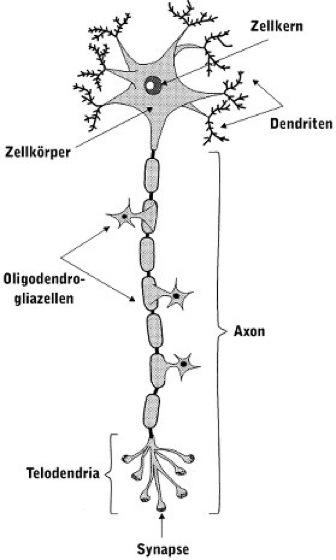
\includegraphics[width=.4\textwidth]{biologisches_neuron.jpg}
	\caption{Aufbau biologisches eines biologischen Neurons (Quelle: \url{https://www.spektrum.de/lexikon/psychologie/neuron/10516})}		\label{fig:BioNeuron}
\end{figure}

Das biologische Neuron (siehe Abb. \ref{fig:BioNeuron}) ist das Vorbild der künstlichen Neuronen. Es besteht aus Dendriten, welche die elektrischen Signale der anderen Neuronen entgegen nehmen und diese an den Zellkörper weiterleiten. 
Am Axonhügel, der zwischen dem Zellkörper und Axon liegt, werden die elektrischen Signale gesammelt und summiert. Erst beim Überschreiten eines gewissen Schwellenwertes, wird das Signal weiter an das Axon geleitet. Durch den Schwellenwert wird verhindert, das sehr kleine Signale weitergeleitet werden, die keine Relevanz haben. Ohne das Filtern der Signale, wäre eine Verarbeitung der relevanten Signale nicht möglich. Das Signal welches letztendlich über das Axon an die Synapsen transportiert wird, heißt Aktionspotential. An die Synapsen schließen andere Dendriten von Neuronen an und empfangen die weitergeleiteten Signale. Ein biologisches Neuron kann dabei bis zu mehreren tausend Verbindungen zu anderen Neuronen besitzen, diese können wieder dementsprechend viele Verbindungen haben.\cite[vgl.][]{Posthoff2022,JuergenCleve2020}

\subsubsection{Künstliches Neuron}
\label{subsubsec:KünstlichesNeuron}
\begin{figure}[ht]
	\centering
	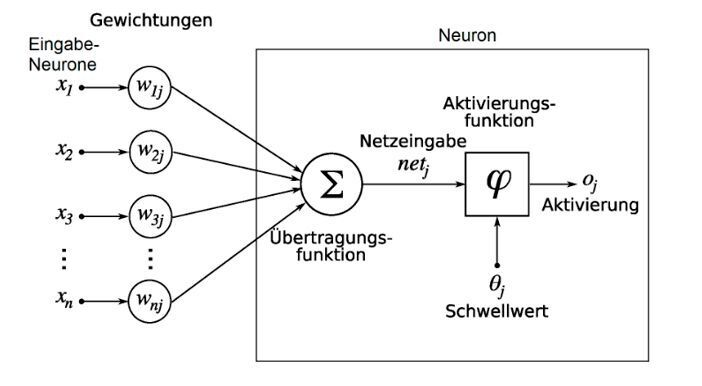
\includegraphics[width=.8\textwidth]{kunstliches_neuron.jpg}
	\caption{Schema eines künstlichen $Neurons_j$ (Quelle: \url{https://www.dev-insider.de/grundbegriffe-und-einfache-beispiele-a-864507/})}
	\label{fig:KünstlichesNeuron}
\end{figure}
Ein künstliches Neuron ist ein mathematisches Modell, das die Funktion eines biologischen Neurons nachahmt. Das künstliche Neuron in Abb. \ref{fig:KünstlichesNeuron} besitzt Eingaben $x_n$, die mit den Dendriten des biologischen Neurons vergleichbar sind. Die Eingabeinformationen können dabei von anderen Neuronen oder aus der Umgebung stammen. \\
Die eingehenden Informationen werden, bevor sie in das Neuron gelangen, mit einer Gewichtung $w_{nj}$ multipliziert. Anschließend werden die Eingaben mithilfe einer Übertragungsfunktion (Propagierungsfunktion) verknüpft, was bedeutet die Werte werden aufsummiert. Das aufsummierte Ergebnis ist die Netzeingabe $net_j$, diese fasst die Informationen zusammen welche in das Neuron gehen. Die Aktivierungsfunktion berechnet die Aktivierung $o_j$, welche je nach Schwellwert $\theta_j$ an alle verbundenen Neuronen weitergeleitet wird. \cite[vgl.][]{JuergenCleve2020}  

\subsubsection{Das Perzeptron}
Ein Perzeptron ist ein einfaches künstliches Neuronales Netz, welches von Frank Rosenblatt als Modell vorgestellt wurde. Als Beispiel wird ein Photo-Perzeptron beschrieben, dass in der Lage ist einfache visuelle Muster zu erkennen. Es besteht aus der Retina (Netzhaut), Assoziationsschicht und der Ausgabeschicht. Die Netzhaut liefert binäre Eingabewerte, welche über gewichtete Verbindungen an die Assoziationsschicht weitergegeben werden. Die Retina Neuronen sind fest mit den Neuronen der Abbildungsschicht verbunden, jedoch sind nicht alle Neuronen miteinander verknüpft. Die Verbindungen zwischen der Abbildungs- und Ausgabeschicht sind hingegen variabel. Während des Trainings, also des Lernens, werden die Gewichtungen  zwischen diesen angepasst. \\
Beim Training werden dem Perzeptron verschiedene Beispiele gezeigt, anhand denen es lernen soll. Ein Beispiel besteht dabei immer aus einem Eingabevektor $x$ und einem Ausgabevektor $y$. Die Aufgabe des Perzeptrons ist es, durch Anpassung der internen Werte zu jedem Eingabevektor $x$, einen passenden Ausgabevektor $y$ zu erzeugen. Das Ziel des Trainings ist es, auf bisher ungesehene, aber ähnliche Eingabevektoren $x'$ ebenfalls einen geeigneten Ausgabevektor $y$ zu assoziieren, in diesem Fall spricht man von einer Generalisierung. \cite[vgl.][]{Scherer1997} \\
Das Perzeptron ist mit seinem Aufbau allerdings beschränkt bei der Klassifikation von Daten. Es ist nur in der Lage linear separierbare Datenmengen zu trennen. Das bedeutet, die Datenmenge kann anhand einer bestimmten Gerade, in zwei separate Datenmengen getrennt werden. Die Ausgaben des Perzeptrons sind also beschränkt auf 0 oder 1, allerdings sind nicht alle Datenmengen trennbar, sondern nur solche deren Trenngerade durch den Ursprung geht.\cite{Ertel2021}

\subsubsection{Aufbau}
Der klassische Aufbau eines Neuronalen Netzes besteht aus einer Eingabeschicht (engl.: Input-Layer), einer oder mehreren versteckten Schichten (engl.: Hidden-Layer), und der Ausgabeschicht (engl.: Output-Layer). Die Eingabeschicht nimmt Werte aus der Umgebung an, und leitet sie weiter an die versteckte Schicht, von wo aus sie an weitere versteckte Schichten oder an die Ausgabeschicht geschickt werden, die das fertige Ergebnis ausgibt. Die Verbindungen der Neuronen zwischen den verschiedenen Schichten besitzen Gewichtungen, mit denen die eingehenden Werte multipliziert werden. Die Komplexität des Aufbaus hängt von der Anzahl der Neuronen und Schichten ab. \cite[vgl.][]{Frochte2020}


\subsubsection{Training eines Neuronalen Netzes}
Das Training eines Neuronalen Netzes ist ein wesentlicher Aspekt des Deep Learnings, bei welchem die Anpassungen der Gewichte und Schwellenwerte innerhalb des Netzwerks stattfinden. Das Training kann oft mehrere Stunden oder sogar Tage dauern, je nach Art und Menge der Daten. Ein Neuronales Netz gilt dann als trainiert, wenn es zu einem Eingabevektor $x$, einen geeigneten Ausgabevekotr $y$ zuverlässig bestimmen kann. Das Netz ist danach in der Lage für bisher ungesehene Eingabevektoren $x'$ ebenfalls passende Ausgabevektoren $y'$ zu zuordnen. \cite[vgl.][]{Scherer1997}

Ein entscheidendes Konzept im Training ist die Fehler- oder Verlustfunktion (engl.: Loss), genauer beschrieben in Abschnitt \ref{subsec:AktivierungsfunktionenVerlust-FunktionenOptimierer}, welche den Unterschied der vorhergesagten Ausgaben mit den tatsächlichen Ergebnissen vergleicht und einen Fehler errechnet. Das Ziel des Trainings ist es, die Verlustfunktion auf ein Minimum zu reduzieren, indem die internen Parameter des Neuronalen Netzes angepasst werden. Die Parameter des Netzwerks werden zu Beginn des Trainings zufällig initialisiert und schrittweise im Training angepasst. \cite[vgl.][]{Choo2020}\\
Die Rückwärtspropagierung (engl.: Backpropagation) ist ein weit verbreitetes Lernverfahren für Neuronale Netze, dass auf eben genannter Minimierung des Fehlers basiert. Für die Rückwärtspropagierung wird im Allgemeinen die Deltalernregel verwendet, die besagt, dass die Fehlerminimierung durch Änderung eines Gewichtes $w_{ij}$ einen Gradientenabstieg bezweckt. Der Ausgangspunkt für diese Lernregel ist wie folgt definiert: 
\begin{equation}
	\Delta_{p}w_{ij} \equiv -\dfrac{dE_p}{dw_{ij}}
\end{equation}
$\Delta_{p}w_{ij}$ entspricht dabei der Änderung eines Gewichts zwischen $i$ und $j$. $dE_p$ ist der gemessene Fehler innerhalb der Lernmenge und $dw_{ij}$ ist die Gewichtung der Neuronen von der Schicht $i$ zur Schicht $j$. \cite[vgl.][]{Rumelhart1986}

Der Backpropagation Algorithmus besteht im wesentlichen aus zwei Schritten, zuerst die Vorwärtspropagierung (engl.: Forwardpropagation) und anschließend die Rückwärtspropagierung.
Der erste Schritt ist die Vorwärtspropagierung, bei dem die Eingabevektoren durch das Netzwerk verarbeitet werden. Die Eingaben werden von Schicht zu Schicht geschickt und durch die Gewichtungen und Aktivierungsfunktionen transformiert. Das Ende dieses Schrittes stellt eine Ausgabe bereit, die dann für den zweiten Schritt weiter verwendet wird. \\
Im nächsten und letzten Schritt des Trainings, der Rückwärtspropagierung, wird die Ausgabe mit dem tatsächlich erwarteten Wert verglichen und anschließend aus der Differenz von Soll- und Ist-Wert ein Fehler errechnet. Als Beispiels Funktion für eine Berechnung eines Fehlers, kann man den mittleren quadratischen Fehler(MSE) verwenden der in \ref{eq:mse} definiert ist.
\begin{equation}
	\label{eq:mse}
	E = \dfrac{1}{2} \sum (Y_i - \hat{Y}_{i})^2
\end{equation}
Nach der Fehlerberechnung, werden die Fehler für die Neuronen der einzelnen Schichten ermittelt. Dabei wird der Beitrag eines jeden Neurons zum Gesamtfehler berechnet. Anschließend wird anhand des Fehlers eines Neurons die Gewichtung von diesem angepasst. Die Gewichte werden dabei mit einem konstanten Faktor $\nu$ und entsprechend des Fehlers mit einem weiteren Term multipliziert. Dieser Prozess wird iterativ wiederholt, bis der Fehler auf ein geeignetes Minimum reduziert wurde. Ist der Fehler auf einen minimalen Wert gesunken und verändert sich nicht mehr großartig, so spricht man davon, dass das \gls{Modell} konvergiert, und das Training beendet werden kann.\cite[vgl.][]{Scherer1997}



\subsection{Aktivierungsfunktionen, Verlust-Funktionen und Optimierer}
\label{subsec:AktivierungsfunktionenVerlust-FunktionenOptimierer}]
Für das Training und die allgemeine Funktionalität eines Neuronalen Netzes sind noch einige Komponenten notwendig.\\
Eine Komponente ist die Aktivierungsfunktion, welche bereits in Abschnitt \ref{subsubsec:KünstlichesNeuron} erwähnt wurde. Sie berechnet die Aktivierung $o_j$, welche in Abhängigkeit eines Schwellwertes $\theta_j$ an die nachgelagerten Neuronen weitergegeben wird. Sollte der Schwellwert $\theta_j$ nicht überschritten werden, wartet das Neuron solange auf weitere Eingabesignale und wiederholt die Berechnung der Aktivierung $o_j$, bis der Schwellwert $\theta_j$ überschritten wird und das Neuron seine Ausgabe weitergibt. Es gibt unterschiedliche Aktivierungsfunktionen für verschiedene Zwecke.

Die Identitätsfunktion ist eine einfache Aktivierungsfunktion und sorgt für eine lineare Abbildung der Eingabe auf die Ausgabe. Diese ist für einfache Aufgaben geeignet, wird die Problemstellung komplexer, so eignen sich mehr nicht-lineare Aktivierungsfunktionen wie der Tangens hyperbolicus, \ac{ReLU} oder Sigmoid. Je nach Anwendung und Bedarf wird eine geeignete Funktion ausgewählt. Die Sigmoid-Funktion normalisiert die Ausgaben eines Netzes auf den Bereich zwischen 0 und 1, während der Tangens hyperbolicus einen die Werte in einen Bereich zwischen -1 und 1 bringt. Die \ac{ReLU}-Funktion verhält sich etwas anders zu den vorangegangen Funktionen, da diese für alle positiven Werte die jeweiligen Ausgaben und für alle negativen Werte den Wert 0 zurückgibt. Eine weitere nennenswerte Aktivierungsfunktion ist die Softmax-Funktion, welche ebenfalls Werte in einen Bereich zwischen 0 und 1 überführt, jedoch aber eine Wahrscheinlichkeitsverteilung darstellt. Die Besonderheit der Softmax-Funktion ist die Gegebenheit, dass sich alle Ausgaben zu 1 addieren und somit die Ausgabewerte als Wahrscheinlichkeiten interpretiert werden können.  \cite[vgl.][]{Frick2021} \\
Eine weitere Komponente ist die Verlust-Funktion, welche essenziell für das Trainieren eines Neuronalen Netzes ist. Diese hat zum Ziel, den Fehler, auch Verlust (engl.: Loss) genannt, den ein Netz bei einer Vorhersage produziert, zu minimieren. Ein Fehler entsteht, wenn das Netz eine falsche oder abweichende Ausgabe als erwartet erzeugt. Um den Gesamtfehler eines Netzes zu berechnen, werden die Ausgaben des Neuronalen Netz mit den erwarteten Ergebnissen verglichen. Die Verlust-Funktion hilft dabei den Unterschied zu quantifizieren und den Gesamtfehler des Netzes zu berechnen. \cite{Frick2021}\\
Wie auch bei den Aktivierungsfunktionen gibt es je nach Art der Aufgabe verschiedene Verlust-Funktionen, wie Binary CrossEntropy (BCE), Categorical Cross Entropy, oder Mean Squared Error. Binary Cross Entropy wird verwendet für binäre Klassifikationsprobleme, wie z.B. das Unterscheiden von seriösen und Spam Emails, währenddessen Categorical Cross Entropy für Probleme mit mehr als zwei Klassen verwendet wird. Die Wahl der Verlust-Funktion hängt dementsprechend auch von der Ausgabe des Netzes ab.   

Die letzte wesentliche Komponente ist der Optimierer (engl.: Optimizer), welcher die Gewichte und Biases anpasst, um den Fehler zu minimieren und die Leistung des Netzes zu verbessern. Biases sind zusätzliche Konstanten, die ein Neuron zugeführt bekommt und bei der Berechnung der Ausgabe eine Rolle spielen. Der Bias erhöht die Fähigkeit des Netzes komplexe Beziehungen zwischen Eingaben und Ausgaben zu modellieren und kann so auch nicht-lineare Zusammenhänge erkennen. \\
Es gibt unterschiedliche Arten von Optimierungsalgorithmen, der am häufigsten verbreitete Algorithmus ist der \ac{SGD}, welcher auch Grundlage für weitere Optimierungsverfahren ist. Der \ac{SGD} aktualisiert Gewichte und Biases basierend auf der Ableitung des Verlustes. Dabei wird eine zufällige Stichprobe aus dem Trainingsdatensatz verwendet, um die Berechnung zu beschleunigen. \cite[vgl.][]{Goodfellow2016} \\
Ein anderer Optimierungsalgorithmus ist Adam, der eine Erweiterung des \ac{SGD} ist und eine adaptive Lernrate verwendet, um die internen Parameter des Netze anzupassen. Der Algorithmus erzielt durch die adaptiven Lernraten eine schnellere Konvergenz und eine höhere Genauigkeit als der \ac{SGD}. \cite[vgl.][]{Kingma2014}

\subsection{\acf{CNN}}
\acf{CNN} sind eine spezielle Form von Neuronalen Netzen, die in der Lage sind Bilddaten zu verarbeiten. Sie erkennen mit verschiedenen Filtern Muster, Strukturen und Geometrien in Bildern und können diese anhand dessen klassifizieren. Im nachfolgenden Abschnitt wird der Aufbau und die Funktionsweise eines \ac{CNN}s erklärt, dabei wird auf die verschiedenen Schichten innerhalb des Netzes, sowie auf die mathematische Operation Faltung (engl.: Convolution) eingegangen.

\begin{figure}[ht]
	\centering
	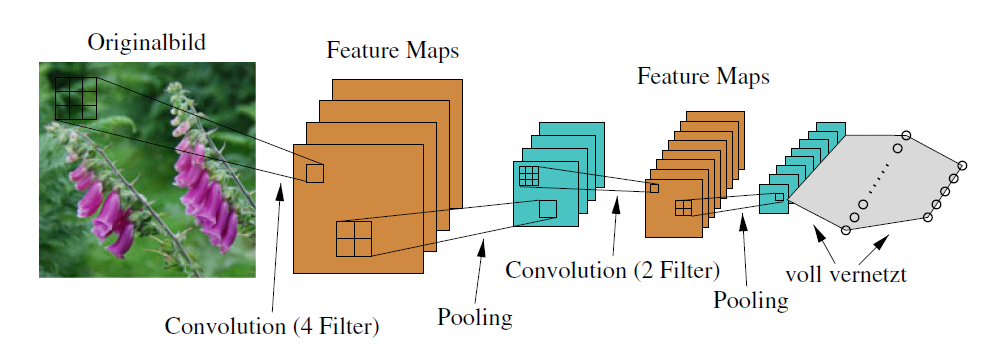
\includegraphics[width=.9\textwidth]{cnn_aufbau.png}
	\caption{Ein \ac{CNN} mit zwei Faltungs-Schichten gefolgt von je einer Pooling-Schicht und am Ende
		zwei voll vernetzten Schichten (Quelle: \cite{Ertel2021})}	
	\label{fig:cnn_aufbau}
\end{figure}

Der Aufbau eines \ac{CNN} besteht aus mehreren Faltungs-Schichten, Pooling-Schichten und voll vernetzten Schichten, wie in Abbildung \ref{fig:cnn_aufbau} zu sehen. 

\paragraph{Convolutional-Layer} ist die Faltungs-Schicht, welche in der Lage ist Merkmale, wie Linien, Kanten und geometrische Formen in Bildern zu erkennen und diese zu extrahieren. Bei einer Faltung wandert ein Filter (engl.: Kernel) über das Eingabebild und erzeugt so ein neues Bild, oder auch sogenannte Feature-Maps. Im mathematischen Sinne gesehen, wandert der Filter über eine Funktion, anstatt über ein Bild und erzeugt somit eine neue. Bei einer Faltung eines Bildes wird meist ein Filter in Form einer 2D-Matrix verwendet, wie er in Gleichung \ref{eq:kernel} als Beispiel zu sehen ist. Die Werte des Filters werden zu Beginn zufällig bestimmt und im Laufe des Trainings angepasst.
\begin{equation}
\begin{bmatrix}
	1 & 2 & 3 \\
	4 & 5 & 6 \\
    7 & 8 & 9
\end{bmatrix}
\label{eq:kernel}
\end{equation}
Der Filter wird schrittweise über das Eingabebild geschoben, wobei jedes Element des Filters mit dem darunterliegendem Bildpunkt des Eingabebildes multipliziert und anschließend aufsummiert wird. Die Summe ist dann das Ergebnis des neuen Bildpunktes. Die Schrittweite des Filters wird als ``Stride'' bezeichnet, und sagt aus, wie viele Bildpunkte, bzw. Pixel, der Filter verschoben wird. Bei einer 2D-Convolution, können zwei Werte für den Stride angegeben werden, die Verschiebung in Richtung der X-Achse und Y-Achse. Die Gleichung \ref{eq:conv_result} zeigt das Ergebnis einer Faltung mit dem Ausdruck aus \ref{eq:conv}.

\begin{equation}
	\begin{pmatrix}
		a_{11} & a_{12} & a_{13} \\
		a_{21} & a_{22} & a_{23} \\
		a_{31} & a_{32} & a_{33}
	\end{pmatrix}
	*
	\begin{pmatrix}
		w_{11} & w_{12} \\
		w_{21} & w_{22}
	\end{pmatrix}
	\label{eq:conv}
\end{equation}

\begin{equation}
	\begin{pmatrix}
		(a_{11}w_{11} + a_{12}w_{12} + a_{21}w_{21} + a_{22}w_{22}) & (a_{12}w_{11} + a_{13}w_{12} + a_{22}w_{21} + a_{23}w_{22}) \\
		(a_{21}w_{11} + a_{22}w_{12} + a_{31}w_{21} + a_{32}w_{22}) & (a_{22}w_{11} + a_{23}w_{12} + a_{32}w_{21} + a_{33}w_{22}) \\
	\end{pmatrix}
	\label{eq:conv_result}
\end{equation}

Es gilt zu beachten, dass das Ergebnis in \ref{eq:conv_result} kleiner ist, als das Ursprungsbild. Dies liegt daran, dass keine Fülldaten (engl.: Padding) verwendet wurde, um die Ränder des Eingabebildes aufzufüllen. Die Größe der Ergebnismatrix lässt sich durch Gleichung \ref{eq:conv_size} berechnen, wobei $W$ die Eingabegröße des Bildes, $F$ die Filtergröße, $S$ der Stride und $P$ das Padding ist. \cite[vgl.][]{Teoh2023}

\begin{equation}
	W_{out}= \dfrac{W+2P-F}{S}+1
	\label{eq:conv_size}
\end{equation}

\paragraph{Pooling-Layer} dient zur Extraktion von Merkmalen (engl.: Features) des Bildes, welche eine hohe semantische Bedeutung haben. Die Eingaben dieser Schicht, sind die Ausgaben der vorangegangenen Faltungs-Schicht. Diese Schicht verwendet entweder das Maximal- oder Mittelwert-Pooling (engl.: Max- oder Average-Pooling). Dabei werden überflüssige und redundante Informationen aus der Datenmenge entfernt. Durch das Entfernen der unwesentlicher Bestandteile reduziert sich Berechnungszeit und die Merkmale werden verdichtet. 

Beim Pooling wandert ebenfalls ein Filter, meist mit einer Größe von $2x2$, und einer Schrittweite von zwei über das Bild. In Abbildung \ref{fig:pooling} werden die zwei Arten des Poolings durchgeführt. Das Max-Pooling extrahiert jeweils den höchsten Wert welcher innerhalb der Filter-Matrix liegt. Das Average-Pooling nimmt jeweils den Mittelwert aller Elemente innerhalb der Filter-Matrix. Durch das Pooling verkleinert sich das Bild je nach Filtergröße und Schrittweite.\cite[vgl.][]{Teoh2023} Im Beispiel von Abbildung \ref{fig:pooling} verkleinert sich das Ausgangsbild um die Hälfte, die Größe nach dem Pooling berechnet sich ebenfalls mit der Formel aus \ref{eq:conv_size}.

\paragraph{Fully-Connected-Layer} oder auch voll verknüpfte Schicht, bildet den Abschluss eines \ac{CNN}s. Die Merkmale der vorangegangenen Schicht, also des Pooling-Layers, werden hier mit allen Ausgabemerkmalen verknüpft, es handelt sich dabei um ein normales Neuronales Netz. 

Zunächst muss aus der Ausgabe der vorangegangenen Schicht eine 1D-Matrix erstellt werden, diesen Prozess nennt man auch ``flatten''. Zuletzt wird schließlich jedes Element aus der 1D-Matrix, mit jedem Element der Ausgabe-Schicht verbunden. Die Ausgabe des Netzes zeigt dann z.B. die Klassifikation eines Bildes, in dem berechnet wird, welches Ausgabeelement die höchste Wahrscheinlichkeit besitzt. \cite[vgl.][]{Weidman2020}

\begin{figure}
	\centering
	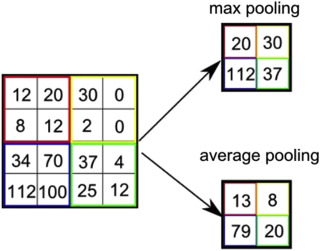
\includegraphics[width=.6\textwidth]{pooling.jpg}
	\caption{Maximal und Mittelwert-Pooling, sowie das Ergebnis der beiden Methoden. (Quelle: \url{https://www.sciencedirect.com/topics/mathematics/pooling-layer})}
	\label{fig:pooling}
\end{figure}


\subsection{Over- und Underfitting}
Over- und Underfitting sind zwei Probleme, die beim Training eines Neuronalen Netzes auftreten können. Diese Probleme beeinflussen die Generalisierungsfähigkeit des Modells, also die Fähigkeit auf neuen und bisher ungesehene Daten gute Ergebnisse zu erzielen.\\
Overfitting tritt auf, wenn sich ein Modell zu stark auf die Trainingsdaten abgestimmt hat und somit keine generelle Strukturen mehr erkennt. Das \gls{Modell} hat sich in diesem Fall die Trainingsdaten gemerkt und kann daher nur schlecht gute Ergebnisse auf neuen Daten erzielen. Ist die Kapazität des \gls{Modell}s zu groß, so neigt das Neuronale Netz dazu kleine Schwankungen in den Daten zu lernen und verliert somit die Generalisierung der Daten.\\
Beim Underfitting hingegen, ist das \gls{Modell} nicht in der Lage eine zugrundeliegende Struktur innerhalb der Daten zu erkennen, was zu einer schlechten Leistung bei den Trainings- und auch bei den Testdaten führt. Im Falle des Underfittings hat das \gls{Modell} meist eine zu geringe Kapazität, um sich alle relevanten Informationen zu speichern.\cite[vgl.][]{Goodfellow2016}